\chapter{Methodology}
\begin{refsection}
 
This chapter discusses the specific steps and logical procedures that was employed to develop and evaluate the Retrieval-Augmented Generation (RAG)-based Large Language Model (LLM) chatbot system. This includes the research design, theoretical and mathematical framework, software and hardware tools, instruments, procedures, evaluation metrics, and a conceptual framework.

\section{Research Design}

This study adopted a constructive research approach, which focuses on designing and building technological artifacts to address real-world problems and evaluating their practical utility \citeauthor{lukka2003cons} \citeyear{lukka2003cons}. This methodology is particularly well-suited to fields like information systems and artificial intelligence, where the goal is not only theoretical insight but also the creation of innovative, functional systems.

In this research, the primary artifact was a Retrieval-Augmented Generation (RAG)-based chatbot integrated with a Large Language Model (LLM). The system was designed to revolutionize how the academe community interacts when finding thesis literature in CSPC library. It addresses the challenges faced in searching and retrieving thesis literature by replacing the current yet traditional database and keyword based search with a vector database and a RAG framework, enabling a conversational and topic-oriented approach. Furthermore, the system was deployed to the cloud, allowing students to access thesis everywhere they are, since current library policies restrict users from taking physical thesis books outside the premises.

% making research faster, smarter, and more user-friendly. It incorporated semantic search using vector embeddings, enabling the RAG chatbot to generate contextually relevant and factually grounded responses for user queries. 

% And also functionalities such as CSPC email authentication for user verification, query history tracking for an improved user experience, and retraining support to adapt to future academic datasets.
% These features highlight the system's real-world relevance, sustainability, and potential for long-term utility \cite{hevner2004design}.

% The system was developed using Streamlit, which allows for the rapid deployment of an interactive user interface. The backend combines vector databases and state-of-the-art LLMs, demonstrating how retrieval and generation components can be effectively integrated to improve access to academic resources. The core data ingestion and experimentation were implemented in a dedicated Jupyter Notebook (\texttt{ingest\_off.ipynb}). This notebook was used to perform structured, token-based chunking aligned with thesis sections, experiment with different embedding models to optimize semantic representation, and visualize the resulting vector space. LangChain was used to orchestrate the final pipeline, with FAISS serving as the vector store for efficient retrieval.


\section{Theorems, Algorithms, and Mathematical Models}

This study implemented advanced machine learning techniques, natural language processing (NLP) models, and the Retrieval-Augmented Generation (RAG) pipeline, integrated with a Large Language Model (LLM) and a vector database. These components collaboratively enabled efficient information retrieval and generation in the context of literature and thesis search within the CSPC Library.

\subsection{Retrieval-Augmented Generation (RAG) Pipeline}

The Retrieval-Augmented Generation (RAG) pipeline is a hybrid architecture that combines information retrieval with natural language generation. It allows LLMs to access external documents during inference, thereby improving both accuracy and contextual relevance.

\begin{figure}[htbp]
    \centering
    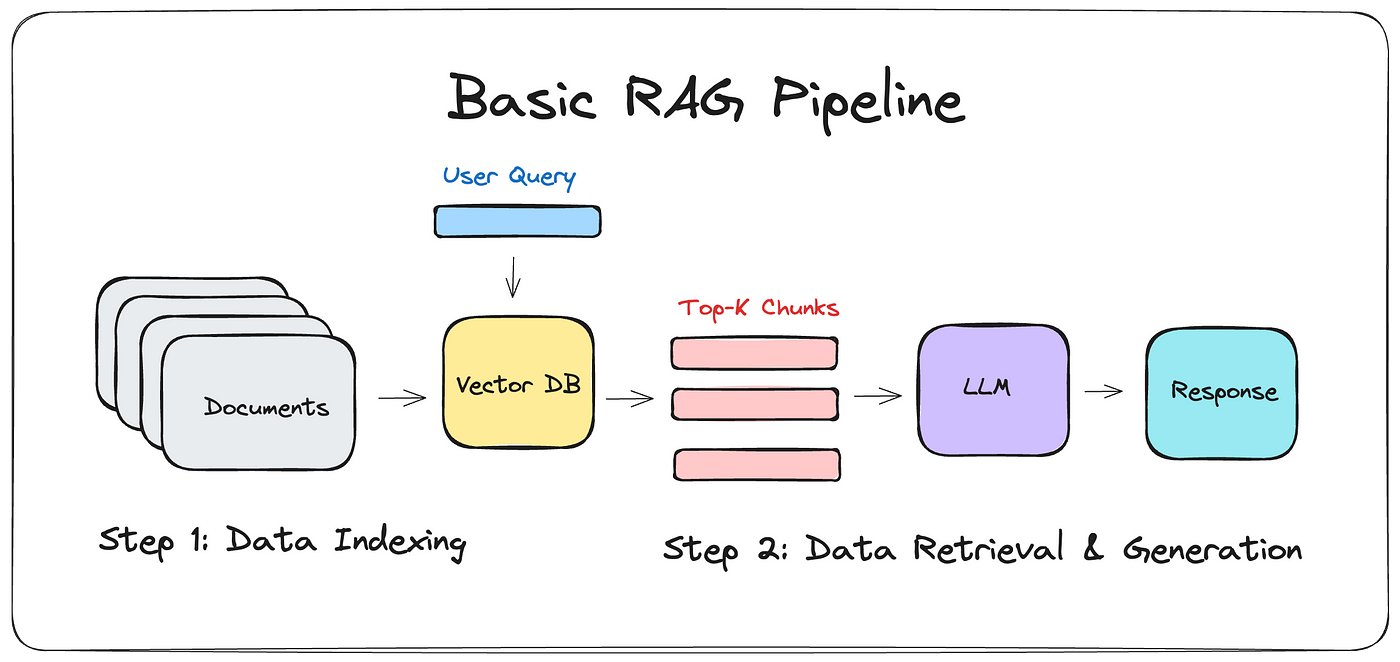
\includegraphics[width=0.7\textwidth]{figures/rag.png}
    \caption{Basic RAG Pipeline by Dr. Julija}
    \label{fig:rag}
\end{figure}

The chatbot’s RAG pipeline, as illustrated in \ref{fig:rag}, consists of the following key stages:

\subsubsection{A. Data Indexing}

The data indexing process begins with document preparation, where thesis documents are collected and preprocessed into smaller, semantically coherent chunks using a token-based method that respects academic structure (e.g., Abstract; Chapters 1–5) to preserve context. Each chunk is then converted into a dense vector using the open-source `sentence-transformers/all-MiniLM-L6-v2` model from Hugging Face, which was chosen for its lightweight architecture and strong semantic representation capabilities. Finally, these vectors and their associated metadata are stored in FAISS, enabling efficient similarity search and scalable retrieval over the entire thesis corpus.

\subsubsection{B. Retrieval and Generation}

The retrieval and generation process begins with query processing, where a user's query is embedded using the same model employed for indexing. A FAISS-backed retriever then performs a semantic search to return the top-$K$ most relevant chunks (default $K=6$), balancing precision and recall. Finally, during contextual generation, these retrieved chunks are provided to the Gemini 2.5-flash language model as grounded context, enabling the generation of relevant and factual responses aligned with the source documents.

\subsection{Large Language Model}

Large Language Models (LLMs) are cutting-edge artificial intelligence systems capable of processing and generating coherent text. These models are built on advanced neural architectures, trained on massive corpora, and have demonstrated effectiveness across NLP tasks such as summarization, question answering, information retrieval, and dialogue systems \citeauthor{naveed2024} \citeyear{naveed2024}. In this study, the system used the Gemini 2.5-flash LLM to synthesize retrieved academic content with its internal knowledge to generate responses tailored to user queries.

\subsubsection{Gemini 2.5-flash}

The large language model integrated in this project is Gemini 2.5 Flash, part of the Gemini 2.X model family introduced by \citeauthor{comanici2025gemini} \citeyear{comanici2025gemini}. Gemini 2.5 Flash delivers advanced reasoning capabilities with support for multimodal inputs, extended context windows, and agentic workflows. Its architecture is optimized to achieve high levels of factual accuracy and contextual relevance while minimizing latency and computational requirements. In this project, Gemini 2.5 Flash was incorporated into a retrieval-augmented generation (RAG) framework to enhance domain-specific information retrieval for CSPC Library users, leveraging its capabilities for real-time, cost-effective, and complex problem-solving.

\section{Materials and Statistical Tools / Evaluation Methods}

To ensure optimal performance of the RAG-based LLM system, several key hardware and software components are required.

\subsection{Instruments}

This section contains the dataset, hardware, and software requirements for the development of the RAG chatbot system.

\subsubsection{Dataset}

The study utilized a dataset consisting of all available undergraduate thesis PDFs from multiple CSPC departments, sourced from the CSPC library. Additionally, the system was designed to ingest newly published theses by allowing admin to upload new PDF files.

\subsubsection{Hardware}

To support the development of RAG chatbot system, the researchers will use hardware components that meet or exceed the specifications outlined in \ref{tab:hardware_requirements}. These components were selected to ensure efficient ingestion of a large corpus of PDFs, as well as to handle computationally intensive tasks like embedding generation.

\begin{table}[H]
    \centering
    \caption{Hardware Requirements}
    \label{tab:hardware_requirements}
    \begin{tabular}{ll}
        \hline
        \textbf{Component}       & \textbf{Specification}                     \\ \hline
        Processor (CPU)          & Modern Multi-core CPU                      \\
        Memory (RAM)             & 16 GB or higher                            \\
        Storage                  & 1 TB SSD or higher                         \\
        Graphics Card (GPU)      & NVIDIA RTX 3090+ (recommended)             \\
        \hline
    \end{tabular}
\end{table}

A modern multi-core CPU enables efficient data processing and model inference, ensuring smooth query execution. At least 16 GB of RAM is recommended to manage large-scale embeddings and real-time retrieval operations effectively. 

A 1 TB SSD is preferred due to its high read/write speeds, which significantly enhance data indexing and retrieval. Given the resource-intensive nature of embedding computations and AI-driven text generation, a high-performance GPU, such as an NVIDIA RTX 3090 or better, is crucial for accelerating deep learning inference and vector operations.

\subsubsection{Software}

\begin{table}[H]
    \centering
    \caption{Software Requirements}
    \label{tab:software_requirements}
    \begin{tabular}{ll}
        \hline
        \textbf{Component}      & \textbf{Specification}                                                               \\ \hline
        Programming Language    & Python 3.10+                                                                         \\
        Vector Database         & e.g. FAISS                                                                           \\
        Language Model          & Gemini 2.5-flash                                                                     \\
        Embedding Model         & \begin{tabular}[c]{@{}l@{}}sentence-transformers/\\ all-MiniLM-L6-v2 (HuggingFace)\end{tabular} \\
        Web Framework           & Streamlit                                                                            \\
        Libraries               & \begin{tabular}[c]{@{}l@{}}LangChain \\ PyMuPDF \\ NumPy \end{tabular} \\
        \hline
    \end{tabular}
\end{table}

Python 3.10 or later serves as the core programming language due to its comprehensive support for machine learning and natural language processing. FAISS is used as the vector database to facilitate fast and accurate semantic search. The system leverages Gemini 2.5-flash as its LLM via the Google Generative AI API, and sentence-transformers/all-MiniLM-L6-v2 to transform preprocessed text chunks into semantically rich vector representations. The Streamlit framework is used to build an interactive user interface.

Document parsing and extraction are managed through the PyMuPDF library, ensuring accurate and efficient retrieval of textual data from PDF files. NumPy supports numerical operations, while LangChain manages the orchestration of LLMs during query interpretation and response generation.


\subsection{Instrument}

The instruments utilized in this study includes 290+ pdf thesis dataset, a vector database, a user evaluation questionnaire, and an automated evaluation toolkit. The dataset consisted of all available PDF thesis documents sourced from the CSPC Library, which were parsed using the PyMuPDF library for text extraction. These documents underwent preprocessing, including cleaning and segmentation into manageable chunks, before being embedded using gemini-embedding-001, a modern embedding model known for its semantic richness and high compatibility with retrieval tasks.

The vectorized representations of these chunks were then stored in FAISS, an open-source vector database optimized for fast similarity search and retrieval, which was vital for the implementation of the RAGAS framework~\cite{trychroma2023chroma}.

A user questionnaire was administered to collect feedback regarding usability, accuracy, and overall satisfaction, utilizing a 5-point Likert scale to ensure consistent measurement.

Survey. Instruments serve as data collection tools across different areas and provide an effective way to gather information. They are useful when seeking insights into the attributes, preferences, opinions, or beliefs of a specific group. To meet the study objectives, the researchers will conduct a survey among employed librarians and CSPC students to evaluate the proposed RAG chatbot using a user-centered method that measures users’ level of agreement on the chatbot’s quality and performance. The researchers will develop questionnaires to assess users’ satisfaction with answers, likelihood to use the chatbot again, ease of reading and understanding the output, and confidence in the information retrieved by the system.

Respondents. The respondents of the study are all from the CSPC including 3 employees of Library, 1 faculty, and the 7 students will serve as a representative of the whole population.

Additionally, the RAGAS (Retrieval-Augmented Generation Assessment Suite) toolkit was utilized to automatically evaluate the quality of system outputs using metrics such as context precision, faithfulness, and answer relevance~\cite{shinn2023ragas}. Furthermore, a context recall metric was included, as recommended for evaluating retrieved chunks. These instruments ensured a rigorous and balanced evaluation of the proposed system from both system-level and user perspectives~ \cite{lin2021bert}.

\section{Statistical Test}

The evaluation of the system utilized the RAGAS framework to evaluate the system's technical performance. It included metrics such as context precision, context recall, answer relevance, and faithfulness. These metrics assessed how accurately the system retrieved and utilized relevant documents to generate responses~\cite{holmes2023chatbot, ameli2024ranking, lin2024satisfaction}.

Additionally, to asssess not only the technical but also the user-centered performance of the system, a user questionnaire was administered to collect feedback regarding usability, accuracy, and overall satisfaction, utilizing a 5-point Likert scale to ensure consistent measurement.

The \ref{tab:likert_scale} shows the description of the 5 Point Likert Scale and the interpretation of the responses. This table shows the corresponding description from the highest to lowest level of agreement.

\begin{table}[H]
    \centering
    \caption{Likert Scale for Chatbot Evaluation}
    \label{tab:likert_scale}
    \begin{tabular}{cccm{7cm}}
        \hline
        \textbf{Scale} & \textbf{Range} & \textbf{Level of Agreement} & \multicolumn{1}{c}{\textbf{Description}} \\
        \hline
                5 & 4.21 - 5.00 & Strongly Agree & The participant strongly supports or agrees with the chatbot's response.\\
        \hline
                4 & 3.21 - 4.20 & Agree & Implies a positive stance toward the chatbot's response. \\
        \hline
                3 & 2.61 - 3.20 & Neutral & The respondent has neither a positive response nor a negative response, but undecided denotes a state of confusion of the respondent. \\
        \hline
                2 & 1.81 - 2.60 & Disagree & Suggests a level of disagreement with the statement or question, but not as strong as Strongly Disagree.\\
        \hline
                1 & 1.00 - 1.80 & Strongly Disagree & Indicates a strong and definitive disagreement with the statement or question. The respondent strongly opposes or disagrees with the chatbot's response.\\
        \hline
    \end{tabular}
\end{table}

Table 3 shows that RAG chatbot system will use 5-point Likert Scale to determine users Level of Agreement based on the user’s experience to the system’s response quality and performance. The first column showed the scale that the system level of agreement fell under which was shown in third column and its corresponding definition in the fourth column. User’s response would be computed using weighted mean and will be determined in which range fell under. Scale 5 with a range of 4.20-5.00 described as “Strongly Agree” which means that the user of the RAG Chatbot completely agrees with the described criteria or finds its quality and performance excellent, scale 4 with a range 3.40-4.19 described as “Agree”, the user of the RAG Chatbot agrees with the described criteria but not to the strongest extent, scale 3 with a range 2.60-3.39 described as “Neutral”, the user of the RAG chatbot is neutral, undecided, or the  criteria description doesn’t strongly resonate in either direction, Scale 2 with a range of 1.80-2.59 described as “Disagree”, the user of the RAG Chatbot disagrees with the criteria description but not as intensely as “Strongly Disagree”, and Scale 1 is described as “Strongly Disagree”, the user of the RAG chatbot completely disagrees with the criteria description or finds the system as low quality and low performance. Another set of questionnaires will be prepared to determine the level of user satisfaction, likelihood of using the application in the future, ease of reading and understanding chatbot output, and confidence in response information regarding the RAG chatbot system. User opinions are expected to provide an understanding of the overall user experience and satisfaction level with the chatbot's performance in thesis retrieval tasks. A Likert scale type of questionnaire will also be used for this purpose, employing the same 5-point scale framework to ensure consistency in measurement and analysis.

In order to analyze the gathered data from the user evaluation questionnaire, the researchers employed the Weighted Mean as the statistical tool. This method was chosen for its effectiveness in summarizing responses on a Likert scale, allowing for a nuanced understanding of user perceptions regarding the chatbot's usability and performance. Also, the level of satisfaction with chatbot answers, likelihood of using the chatbot again, ease of reading and understanding the output, and users’ confidence in the accuracy of the chatbot’s responses will be evaluated:

\begin{equation}
    \centering
    WM = \frac{TWM}{N}
\end{equation}

Where:
\begin{itemize}
    \item $WM$ = Weighted Mean
    \item $TWM$ = Total Weighted Mean
    \item $N$ = Total number of respondents
\end{itemize}

\section{Procedures}

The procedures encompassed the collection and preprocessing of academic data, vector-based indexing, retrieval using semantic search, LLM-based response generation, and multi-metric evaluation using RAGAS, and user-centered evaluation.

Each stage was designed to ensure the integrity, replicability, and effectiveness of the system in addressing the research objectives. By detailing the technical and methodological steps, this section served as a transparent and structured guide for future researchers seeking to replicate or build upon this study.

% \subsection*{Data Collection}

% PDF thesis documents were gathered from CSPC Library’s digital archives, focusing on undergraduate theses and institutional research. The collection process ensured that documents were academically relevant and representative of typical user queries.

\begin{enumerate}

    \item \textbf{Data Preprocessing} - 
        \begin{enumerate}
            \item [(a)] {Text Extraction:} PyMuPDF was used to convert PDF files into structured plain text.
            \item [(b)] {Cleaning:} Non-informative characters and formatting were removed.
            \item [(c)] {Text Chunking:} Text was segmented into manageable chunks to enhance semantic search accuracy.
        \end{enumerate}
        
    \item \textbf{Indexing and Vector Embedding} - 
        \begin{enumerate}
            \item [(a)] {Vector Embedding:} Each text chunk will be embedded using gemini-embedding-001.
            \item [(b)] {Cleaning:} FAISS will store the vectorized content along with metadata such as document titles, authors, and section headers.
        \end{enumerate}

    \item \textbf{Query Handling and Semantic Retrieval} - 
        \begin{enumerate}
            \item [(a)] {Query Encoding:} The user’s natural language query is encoded using the same embedding model applied during indexing to maintain compatibility in the latent space.
            \item [(b)] {Similarity Search:} The encoded query is matched against stored vectors to retrieve the top-$K$ relevant chunks (default $K=6$). For exploratory or synthesis-oriented queries, $K$ may be adaptively increased to improve coverage.
        \end{enumerate}

    \item \textbf{Response Generation} - The Gemini 2.5-flash language model will process the augmented input to generate a response that is factually aligned with the source documents.

    \item \textbf{Output Presentation} - The system will display the generated response via a user interface that includes metadata such as the source thesis title and section, encouraging transparency and academic integrity.

    \item \textbf{Performance Evaluation} - 
        \begin{enumerate}
            \item [(a)] {Automated Evaluation:} Metrics from the RAGAS framework, Context Precision, Context Recall, Answer Relevance, and Faithfulness, will be calculated.
            \item [(b)] {Human Evaluation:} A usability questionnaire was distributed to a sample of student users to assess the system’s clarity, ease of use, and usefulness in retrieving academic information.
        \end{enumerate}

\end{enumerate}


\section{Evaluation Metrics}

The researchers used a framework called \textbf{RAGAS} that comprised specific metrics to assess Retrieval-Augmented Generation (RAG)-based architectures, thereby ensuring precise measurements of both retrieval quality and generation fidelity~\cite{oubah2024advanced}. This framework evaluated the model's performance using the following metrics: \textit{Context Precision}, \textit{Context Recall}, \textit{Response Relevance}, and \textit{Faithfulness}. Each metric was essential in addressing the system’s retrieval and generation performance.

\subsection*{Context Precision}

The Context Precision metric was used to evaluate the retrieval quality of the RAG chatbot within the CSPC Library. It measured the proportion of relevant document chunks among the top $K$ retrieved results, emphasizing the system's ability to present highly relevant content at higher ranks. A higher Context Precision indicated that the system effectively prioritized relevant information for the user.

\begin{equation}
\centering
\text{Context Precision@K} = 
\frac{
    \sum_{k=1}^{K} \left( \text{Precision@k} \times v_k \right)
}{
    \text{Total number of relevant items in the top } K \text{ results}
}
\end{equation}

where $\text{Precision@k}$ is the precision at rank $k$, and $v_k$ is a binary indicator variable such that $v_k = 1$ if the chunk at position $k$ is relevant, and $v_k = 0$ otherwise. Here, $K$ indicates the cutoff for the top results evaluated. The denominator normalizes the metric by accounting for the total number of relevant items within the top $K$ retrieved results. This weighted approach ensures that relevant items retrieved earlier in the ranking contribute more significantly to the final score, making the metric especially meaningful for library retrieval tasks.

The precision at each position $k$, denoted as Precision@k, is computed as follows:

\begin{equation}
\centering
\text{Precision@k} = 
\frac{
    \text{true positives@k}
}{
    \text{true positives@k} + \text{false positives@k}
}
\end{equation}

where $\text{true positives@k}$ is the number of relevant chunks retrieved up to position $k$, and $\text{false positives@k}$ is the number of non-relevant chunks retrieved up to the same position. This component metric quantifies retrieval accuracy at each rank and serves as a foundation for the overall Context Precision@K calculation.

\subsection*{Context Recall}

Context Recall was used to evaluate the comprehensiveness of the retrieval system in capturing all relevant information necessary to answer a query. It measured the proportion of relevant chunks successfully retrieved by the RAG chatbot within the CSPC Library, ensuring minimal omission of important academic content.

\begin{equation}
\centering
\text{Context Recall} = \frac{\text{Number of relevant claims supported by retrieved chunks}}{\text{Total number of relevant claims in the reference answer}}
\end{equation}

where:

\begin{itemize}
    \item \textit{Number of relevant claims supported by retrieved chunks} refers to the count of factual claims in the ground truth answer that can be attributed to the retrieved document chunks,
    \item \textit{Total number of relevant claims in the reference answer} represents all the factual claims present in the ground truth answer that ideally should be covered by the retrieval process.
\end{itemize}

This metric captures how effectively the system covers the necessary knowledge, with a value ranging between 0 and 1, where 1 indicates perfect recall. It ensures that critical academic information is not missed during retrieval, making it an essential part of evaluating the RAG chatbot system.


\subsection*{Response Relevance}

Response Relevance was a critical metric used to evaluate how well the RAG chatbot's generated answer addressed the specific query posed by users in the CSPC Library. This metric ensured that the chatbot provided focused, comprehensive, and directly applicable responses to academic inquiries, minimizing irrelevant or incomplete information that could hinder research efficiency.

\begin{equation}
\centering
\text{Response Relevance} = \frac{1}{N} \sum_{i=1}^{N} \cos(E_{g_i}, E_o)
\end{equation}

where:
\begin{itemize}
    \item $N$ is the number of artificially generated questions based on the response (typically 3),
    \item $E_{g_i}$ is the embedding of the $i$-th generated question derived from the response,
    \item $E_o$ is the embedding of the original user query,
    \item $\cos(E_{g_i}, E_o)$ represents the cosine similarity between the generated question embedding and the original query embedding.
\end{itemize}

This metric works on the idea that if the chatbot's response sufficiently answers the original query, then questions generated from that response will semantically align with the original question, this involves generating multiple artificial questions, embedding both the response-generated questions and the original query into vector representations, and calculating the mean cosine similarity to measure alignment, which ensures that the retrieved academic information closely matches the research needs of CSPC Library users.

\subsection*{Faithfulness}

Faithfulness is a critical metric for evaluating the factual consistency of the RAG chatbot's generated responses with respect to the retrieved context from the CSPC Library. This metric ensures that all claims made in the chatbot's answer are directly supported by the information present in the retrieved documents, thereby minimizing hallucinations and maintaining academic integrity.

\begin{equation}
\centering
\text{Faithfulness} = \frac{\text{Number of claims in the response supported by retrieved context}}{\text{Total number of claims in the response}}
\end{equation}

where:
\begin{itemize}
\item \textit{Number of claims in the response supported by retrieved context} refers to the count of factual statements in the generated answer that can be directly verified or inferred from the retrieved context chunks,
\item \textit{Total number of claims in the response} is the complete count of all factual statements made in the answer, regardless of whether they are supported by the context.
\end{itemize}

A faithfulness score of $1.0$ indicates that all claims in the response are grounded in the retrieved context, while lower scores reveal the presence of unsupported or hallucinated information. In the context of academic literature search and thesis retrieval, maintaining high faithfulness is essential to ensure that the chatbot's answers are trustworthy and factually accurate, directly reflecting the content of the CSPC Library's resources.


\section{Conceptual Framework}

The conceptual framework served as the foundational blueprint for the RAG-based chatbot system. It emphasized the end-to-end interaction of modules required to support intelligent, accurate, and efficient academic document retrieval. As illustrated in \ref{fig:conceptual_framework}, the system followed a cyclical process beginning with data collection and ending with system evaluation and refinement.
The arrows were used solely to visually indicate the step-by-step flow of each component within the chatbot framework; they did not signify any technical operation or special relationship beyond showing the direction of the process. 

This visualization helps guide readers through the sequence of the system stages, ensuring clarity at the outset.

\begin{figure}[H]
    \centering
    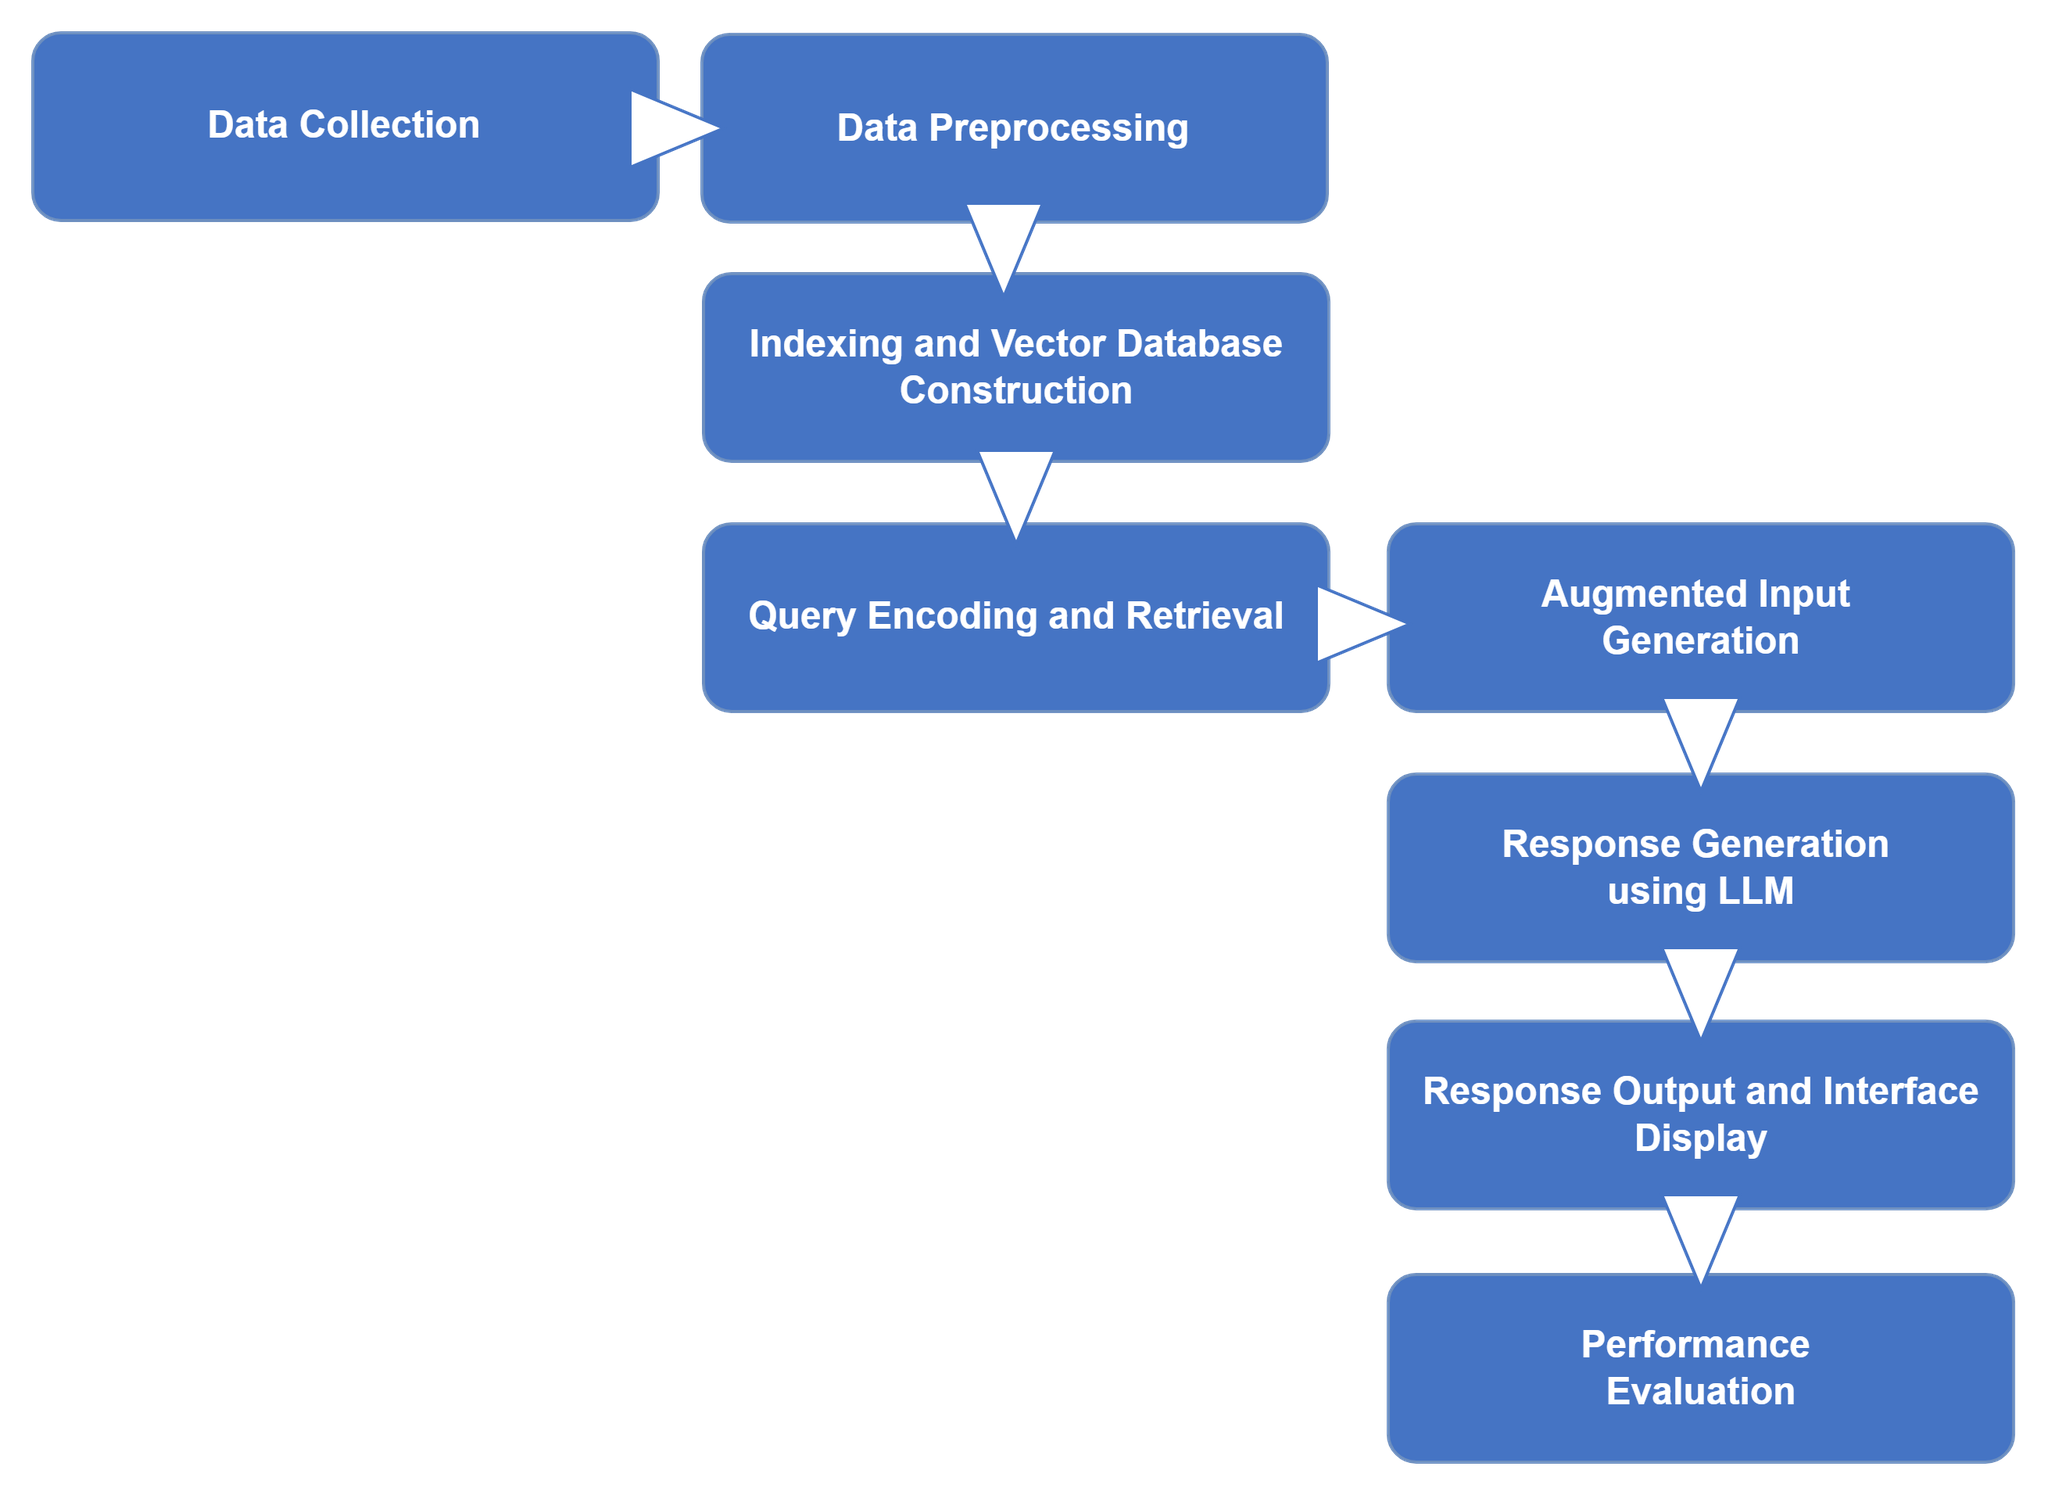
\includegraphics[width=0.7\textwidth]{figures/framework.png}
    \caption{Conceptual Framework of the RAG-Based Chatbot System}
    \label{fig:conceptual_framework}
\end{figure}

The process began with \textbf{data collection}, where PDF-format academic documents such as undergraduate theses and institutional research papers were sourced from the CSPC Library’s digital repository. These documents formed the primary knowledge base of the system.

In the \textbf{data pre-processing} phase, tools like PyMuPDF were used to extract plain text from the collected PDFs. The extracted content underwent cleaning and normalization to remove non-informative characters, followed by segmentation into semantically meaningful text chunks.

Next, the system performed \textbf{model training}, where embedding models such as gemini embeddings were used to transform the text chunks into vector representations.


These embeddings preserved the semantic meaning of the documents and prepared them for storage and retrieval.

The \textbf{input sampling} stage supported the gathering and simulation of user queries. These sample inputs reflected typical academic inquiries posed by students when searching for specific thesis content.

In the \textbf{input pre-processing} phase, user queries were tokenized and encoded using the same embedding model applied during training. This enabled semantic similarity comparison between the user query and the pre-embedded document vectors.

The system then proceeded to \textbf{location mapping}, which corresponded to the semantic search function performed using FAISS. Here, the system retrieved the top-K most relevant document chunks by measuring vector similarity.

During \textbf{model inference}, an augmented input was created by combining the user query with the retrieved chunks. This augmented prompt was forwarded to a generative language model (e.g., Gemini 2.5-flash) to produce a contextually grounded response aligned with the original academic documents.

Finally, \textbf{performance evaluation} was conducted using a dual-layer assessment. System-level performance was measured using the RAGAS framework with metrics such as Context Precision, Context Recall, Answer Relevance and Faithfulness. This framework ensured that each component of the RAG-based chatbot system operated in coordination, contributing to a reliable and academically useful tool for thesis retrieval and literature assistance.

%=======================================================%
%%%%% Do not delete this part %%%%%%
\clearpage

\printbibliography[heading=subbibintoc, title={\centering Notes}]
\end{refsection}
